\documentclass[a4paper,10pt]{article}\setlength{\textheight}{10in}\setlength{\textwidth}{6.5in}\setlength{\topmargin}{-0.125in}\setlength{\oddsidemargin}{-.2in}\setlength{\evensidemargin}{-.2in}\setlength{\headsep}{0.2in}\setlength{\footskip}{0pt}\usepackage{amsmath}\usepackage{fancyhdr}\usepackage{enumitem}\usepackage{hyperref}\usepackage{xcolor}\usepackage{graphicx}\pagestyle{fancy}

\lhead{Name: \rule{5cm}{0.5pt}}
\chead{M.Number: \rule{2cm}{0.5pt}}
\rhead{KDDM1 VO (INP.31101UF)}
\fancyfoot{}

\begin{document}
\begin{enumerate}[topsep=0mm, partopsep=0mm, leftmargin=*]

{\color{blue}
\item\textit{Visual Data Analysis}. Given the dataset ``visual-dataset.csv'' (available in TeachCenter), which comprises a number of features and a binary target feature.
\begin{enumerate}
	\item Provide a number of meaningful visualisations (3-5 visualisations)
	\item Based on the visualisations provide your key interpretation on
	\begin{enumerate}
		\item Are there noteworthy dependencies between the features?
		\item What types of dependency/relationship are there?
		\item Are we expecting the prediction to work well?
	\end{enumerate}
\end{enumerate}
}

%%% Your answer here

{\color{blue}
\newpage\item\textit{Correlation}. Given a dataset, which consists of 1,000 variables (hint: most of them are just random), the goal is to find the relationships between variables, i.e., which and how do the variables relate to each other; what are the dependencies.
The dataset ``correlation-dataset.csv'' can be downloaded from TeachCenter.
\begin{enumerate}
	\item Which methods did you apply to find the relationships, and why?
	\item Which relationships did you find and how do you characterise the relationships (e.g., variable ``Michael'' to ``Christopher'' is linear)?
	\item Which causal relationships between the variables can you find (e.g., variable ``Jessica'' causes ``Matthew'')?
\end{enumerate}
}

%%% Your answer here



{\color{blue}
\newpage\item \textit{Outliers/Anomalies}. 
\begin{enumerate}
\item For both data sets shown below define yourself, what is the normal behaviour and what are the outliers/anomalies, please indicate in the image the anomalous behaviour
\item Name the algorithms or describe the algorithmic way of how to identify this anomalous behaviour (you may choose different algorithms for each data set, also describe any necessary preprocessing)
\item Name the assumptions made by your algorithms
\end{enumerate}
\begin{center}
 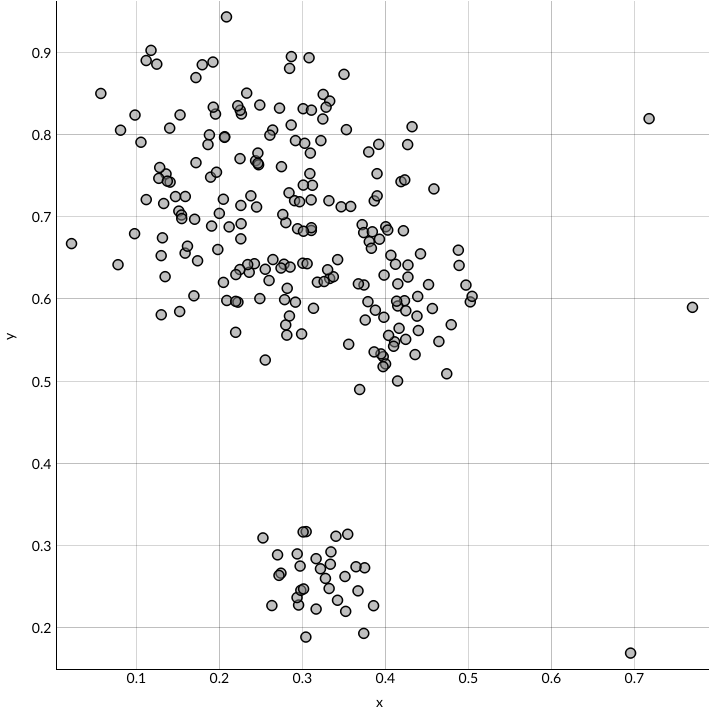
\includegraphics[width=.4\textwidth]{outlier-dataset-1.png}
 \hspace{2cm}
 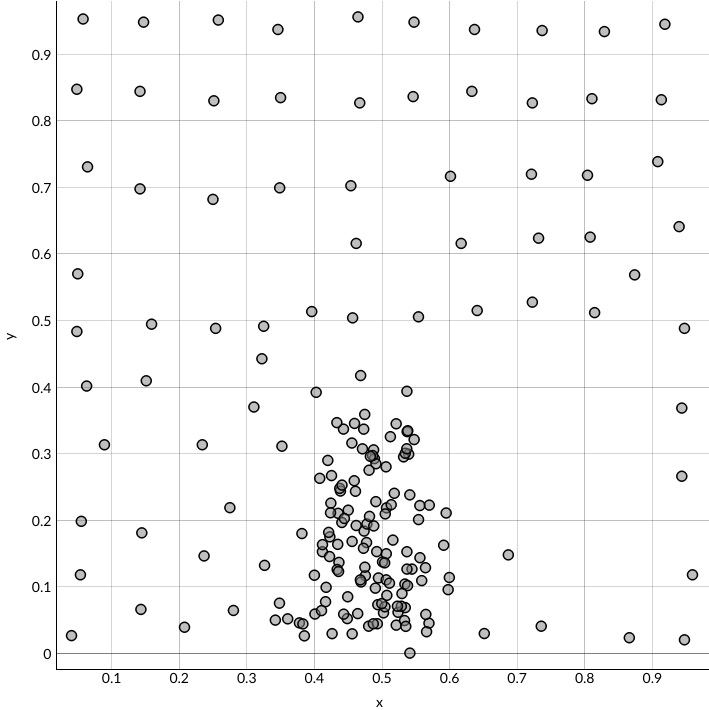
\includegraphics[width=.4\textwidth]{outlier-dataset-2.png}
\end{center}
}

%%% Your answer here



{\color{blue}
\newpage\item\textit{Missing Values}. The dataset ``missing-values-dataset.csv'' (available on TeachCenter) contains a number of missing values.
\begin{enumerate}
	\item Try to reconstruct why the missing values are missing? What could be an explanation?
	\item What methods do you apply?
	\item What strategies are applicable for the features to deal with the missing values?
	\item For each feature provide an estimate of the arithmetic mean (of the version of the dataset without missing values)?
\end{enumerate}
}

%%% Your answer here

\end{enumerate}
\end{document}
